% Created by tikzDevice version 0.12.3 on 2020-04-18 10:16:28
% !TEX encoding = UTF-8 Unicode
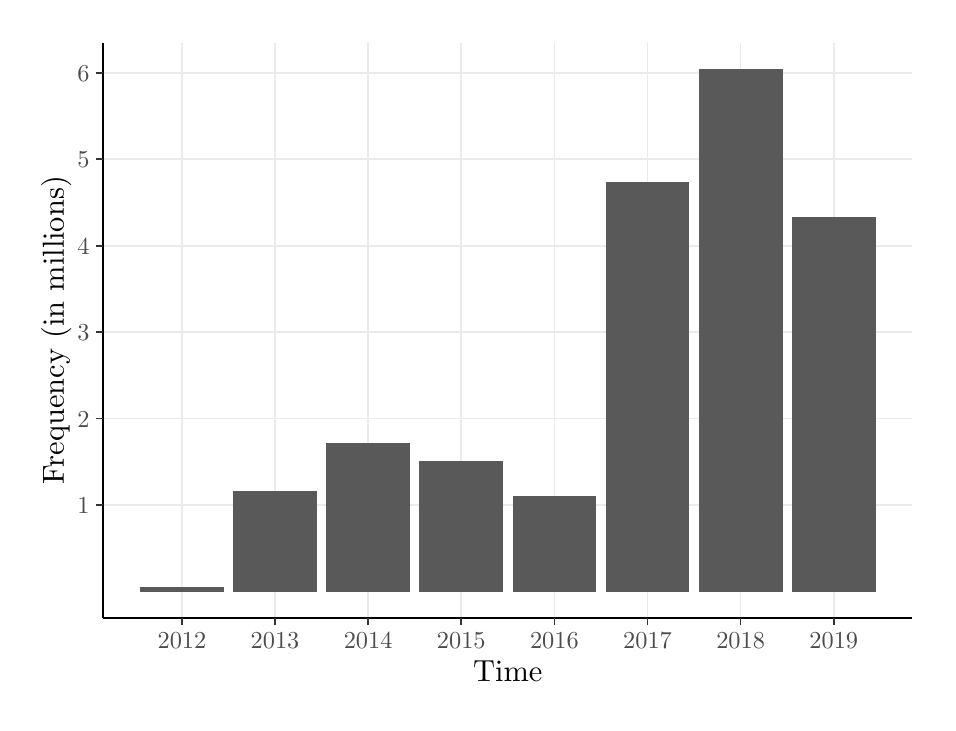
\begin{tikzpicture}[x=1pt,y=1pt]
\definecolor{fillColor}{RGB}{255,255,255}
\path[use as bounding box,fill=fillColor,fill opacity=0.00] (0,0) rectangle (325.21,243.91);
\begin{scope}
\path[clip] (  0.00,  0.00) rectangle (325.21,243.91);
\definecolor{drawColor}{RGB}{255,255,255}
\definecolor{fillColor}{RGB}{255,255,255}

\path[draw=drawColor,line width= 0.6pt,line join=round,line cap=round,fill=fillColor] (  0.00,  0.00) rectangle (325.21,243.91);
\end{scope}
\begin{scope}
\path[clip] ( 27.31, 30.69) rectangle (319.71,238.41);
\definecolor{fillColor}{RGB}{255,255,255}

\path[fill=fillColor] ( 27.31, 30.69) rectangle (319.71,238.41);
\definecolor{drawColor}{gray}{0.92}

\path[draw=drawColor,line width= 0.6pt,line join=round] ( 27.31, 71.38) --
	(319.71, 71.38);

\path[draw=drawColor,line width= 0.6pt,line join=round] ( 27.31,102.63) --
	(319.71,102.63);

\path[draw=drawColor,line width= 0.6pt,line join=round] ( 27.31,133.88) --
	(319.71,133.88);

\path[draw=drawColor,line width= 0.6pt,line join=round] ( 27.31,165.13) --
	(319.71,165.13);

\path[draw=drawColor,line width= 0.6pt,line join=round] ( 27.31,196.38) --
	(319.71,196.38);

\path[draw=drawColor,line width= 0.6pt,line join=round] ( 27.31,227.63) --
	(319.71,227.63);

\path[draw=drawColor,line width= 0.6pt,line join=round] ( 55.75, 30.69) --
	( 55.75,238.41);

\path[draw=drawColor,line width= 0.6pt,line join=round] ( 89.39, 30.69) --
	( 89.39,238.41);

\path[draw=drawColor,line width= 0.6pt,line join=round] (123.04, 30.69) --
	(123.04,238.41);

\path[draw=drawColor,line width= 0.6pt,line join=round] (156.69, 30.69) --
	(156.69,238.41);

\path[draw=drawColor,line width= 0.6pt,line join=round] (190.34, 30.69) --
	(190.34,238.41);

\path[draw=drawColor,line width= 0.6pt,line join=round] (223.99, 30.69) --
	(223.99,238.41);

\path[draw=drawColor,line width= 0.6pt,line join=round] (257.63, 30.69) --
	(257.63,238.41);

\path[draw=drawColor,line width= 0.6pt,line join=round] (291.28, 30.69) --
	(291.28,238.41);
\definecolor{fillColor}{gray}{0.35}

\path[fill=fillColor] ( 40.60, 40.13) rectangle ( 70.89, 41.72);

\path[fill=fillColor] ( 74.25, 40.13) rectangle (104.54, 76.56);

\path[fill=fillColor] (107.90, 40.13) rectangle (138.18, 93.65);

\path[fill=fillColor] (141.55, 40.13) rectangle (171.83, 87.49);

\path[fill=fillColor] (175.20, 40.13) rectangle (205.48, 74.68);

\path[fill=fillColor] (208.84, 40.13) rectangle (239.13,188.20);

\path[fill=fillColor] (242.49, 40.13) rectangle (272.78,228.97);

\path[fill=fillColor] (276.14, 40.13) rectangle (306.42,175.66);
\end{scope}
\begin{scope}
\path[clip] (  0.00,  0.00) rectangle (325.21,243.91);
\definecolor{drawColor}{RGB}{0,0,0}

\path[draw=drawColor,line width= 0.6pt,line join=round] ( 27.31, 30.69) --
	( 27.31,238.41);
\end{scope}
\begin{scope}
\path[clip] (  0.00,  0.00) rectangle (325.21,243.91);
\definecolor{drawColor}{gray}{0.30}

\node[text=drawColor,anchor=base east,inner sep=0pt, outer sep=0pt, scale=  0.88] at ( 22.36, 68.35) {1};

\node[text=drawColor,anchor=base east,inner sep=0pt, outer sep=0pt, scale=  0.88] at ( 22.36, 99.60) {2};

\node[text=drawColor,anchor=base east,inner sep=0pt, outer sep=0pt, scale=  0.88] at ( 22.36,130.85) {3};

\node[text=drawColor,anchor=base east,inner sep=0pt, outer sep=0pt, scale=  0.88] at ( 22.36,162.10) {4};

\node[text=drawColor,anchor=base east,inner sep=0pt, outer sep=0pt, scale=  0.88] at ( 22.36,193.35) {5};

\node[text=drawColor,anchor=base east,inner sep=0pt, outer sep=0pt, scale=  0.88] at ( 22.36,224.60) {6};
\end{scope}
\begin{scope}
\path[clip] (  0.00,  0.00) rectangle (325.21,243.91);
\definecolor{drawColor}{gray}{0.20}

\path[draw=drawColor,line width= 0.6pt,line join=round] ( 24.56, 71.38) --
	( 27.31, 71.38);

\path[draw=drawColor,line width= 0.6pt,line join=round] ( 24.56,102.63) --
	( 27.31,102.63);

\path[draw=drawColor,line width= 0.6pt,line join=round] ( 24.56,133.88) --
	( 27.31,133.88);

\path[draw=drawColor,line width= 0.6pt,line join=round] ( 24.56,165.13) --
	( 27.31,165.13);

\path[draw=drawColor,line width= 0.6pt,line join=round] ( 24.56,196.38) --
	( 27.31,196.38);

\path[draw=drawColor,line width= 0.6pt,line join=round] ( 24.56,227.63) --
	( 27.31,227.63);
\end{scope}
\begin{scope}
\path[clip] (  0.00,  0.00) rectangle (325.21,243.91);
\definecolor{drawColor}{RGB}{0,0,0}

\path[draw=drawColor,line width= 0.6pt,line join=round] ( 27.31, 30.69) --
	(319.71, 30.69);
\end{scope}
\begin{scope}
\path[clip] (  0.00,  0.00) rectangle (325.21,243.91);
\definecolor{drawColor}{gray}{0.20}

\path[draw=drawColor,line width= 0.6pt,line join=round] ( 55.75, 27.94) --
	( 55.75, 30.69);

\path[draw=drawColor,line width= 0.6pt,line join=round] ( 89.39, 27.94) --
	( 89.39, 30.69);

\path[draw=drawColor,line width= 0.6pt,line join=round] (123.04, 27.94) --
	(123.04, 30.69);

\path[draw=drawColor,line width= 0.6pt,line join=round] (156.69, 27.94) --
	(156.69, 30.69);

\path[draw=drawColor,line width= 0.6pt,line join=round] (190.34, 27.94) --
	(190.34, 30.69);

\path[draw=drawColor,line width= 0.6pt,line join=round] (223.99, 27.94) --
	(223.99, 30.69);

\path[draw=drawColor,line width= 0.6pt,line join=round] (257.63, 27.94) --
	(257.63, 30.69);

\path[draw=drawColor,line width= 0.6pt,line join=round] (291.28, 27.94) --
	(291.28, 30.69);
\end{scope}
\begin{scope}
\path[clip] (  0.00,  0.00) rectangle (325.21,243.91);
\definecolor{drawColor}{gray}{0.30}

\node[text=drawColor,anchor=base,inner sep=0pt, outer sep=0pt, scale=  0.88] at ( 55.75, 19.68) {2012};

\node[text=drawColor,anchor=base,inner sep=0pt, outer sep=0pt, scale=  0.88] at ( 89.39, 19.68) {2013};

\node[text=drawColor,anchor=base,inner sep=0pt, outer sep=0pt, scale=  0.88] at (123.04, 19.68) {2014};

\node[text=drawColor,anchor=base,inner sep=0pt, outer sep=0pt, scale=  0.88] at (156.69, 19.68) {2015};

\node[text=drawColor,anchor=base,inner sep=0pt, outer sep=0pt, scale=  0.88] at (190.34, 19.68) {2016};

\node[text=drawColor,anchor=base,inner sep=0pt, outer sep=0pt, scale=  0.88] at (223.99, 19.68) {2017};

\node[text=drawColor,anchor=base,inner sep=0pt, outer sep=0pt, scale=  0.88] at (257.63, 19.68) {2018};

\node[text=drawColor,anchor=base,inner sep=0pt, outer sep=0pt, scale=  0.88] at (291.28, 19.68) {2019};
\end{scope}
\begin{scope}
\path[clip] (  0.00,  0.00) rectangle (325.21,243.91);
\definecolor{drawColor}{RGB}{0,0,0}

\node[text=drawColor,anchor=base,inner sep=0pt, outer sep=0pt, scale=  1.10] at (173.51,  7.64) {Time};
\end{scope}
\begin{scope}
\path[clip] (  0.00,  0.00) rectangle (325.21,243.91);
\definecolor{drawColor}{RGB}{0,0,0}

\node[text=drawColor,rotate= 90.00,anchor=base,inner sep=0pt, outer sep=0pt, scale=  1.10] at ( 13.08,134.55) {Frequency (in millions)};
\end{scope}
\end{tikzpicture}
